%%%%%%%%%%%%%%%%%%%%%%%%%%%%%%%%%%%%%%%%%%%%%%%%%%%%%%%%%%%%%%%
% IDEA Cipher
% David Miguel Lozano
% Warszawa - 2016
%%%%%%%%%%%%%%%%%%%%%%%%%%%%%%%%%%%%%%%%%%%%%%%%%%%%%%%%%%%%%%%

% -------------------------------------------------------------
% Preamble
% -------------------------------------------------------------
\documentclass[a4paper,12pt,titlepage]{article}

% -------------------------------------------------------------
% Packages
% -------------------------------------------------------------
\usepackage[utf8]{inputenc}	% Unicode support
\usepackage[T1]{fontenc} 		% Font encoding
\usepackage[english]{babel}	% Languaje
\usepackage{lmodern} 	% Typeface 
\usepackage{graphicx}	% Add pictures
\usepackage{hyperref}	% Add a link to index entries
\usepackage{amsmath} 	% Advanced math typesetting
\usepackage{amsfonts}	% Mathematical formulas
\usepackage{amssymb}	% Extended symbol collection
\usepackage{listings} % Code formatting and highlighting
\usepackage{xcolor}		% Color package
\usepackage{enumitem} % Customizing lists
\usepackage{parskip}	% Paragraph styles
\usepackage[numbers,sort]{natbib} % Bibliography management 

% -------------------------------------------------------------
% Configuration
% -------------------------------------------------------------
% Images path
\graphicspath{ {images/} }
% Hyperlinks coloring
\hypersetup{
	colorlinks,
	linkcolor={green!40!black},
	citecolor={blue!50!black},
	urlcolor={blue!80!black}
}
% Define HRule
\newcommand{\HRule}[1]{\rule{\linewidth}{#1}}

\begin{document}
% -------------------------------------------------------------
% Cover
% -------------------------------------------------------------
\author{David Miguel Lozano}
\title{IDEA cipher}
\date{11-05-2016}

\begin{titlepage}
	\centering
	
\includegraphics[width=0.2\textwidth]{images/pw-logo.png}\par
	\vspace{0.3cm}
	{\scshape\LARGE Politechnika Warszawska \par}
	\vfill
	{\scshape\Large Cryptography and Information Security \par}
	\HRule{2pt}
	{\huge\bfseries IDEA cipher \par}
	\HRule{2pt}
	\\ [0.5cm]
	{Software implementation of International Data Encryption Algorithm (IDEA) cipher with 4 ciphering modes.}
	\vfill
	Student:\par
	{\Large\scshape David Miguel Lozano \par}
	\vfill
	Guided by:\par
	Dr.~Tomasz \textsc{Adamski}
	\vfill
	{\large Summer 2016 \par}
\end{titlepage}

% -------------------------------------------------------------
% Contents
% -------------------------------------------------------------
\newpage
\tableofcontents
\begin{appendix}
  \listoffigures
  %\listoftables
\end{appendix}

% -------------------------------------------------------------
% Body
% -------------------------------------------------------------
\newpage

\section{Introduction}

The purpose of this report is to introduce the International Data Encryption Algorithm (IDEA) and describe the implementation done.

"International Data Encryption Algorithm (IDEA), originally called Improved Proposed Encryption Standard (IPES), is a symmetric-key block cipher designed by James Massey of ETH Zurich and Xuejia Lai and was first described in 1991. The algorithm was intended as a replacement for the Data Encryption Standard (DES). IDEA is a minor revision of an earlier cipher, Proposed Encryption Standard (PES)."  \citep{wiki:idea}

\section{Symmetric-key algorithm}

A symmetric key algorithm is a cryptography algorithm that use the same key for encryption and decryption. This key is a shared secret between the different parties that want to keep some secret information. \citep{wiki:symmetric-key}

\paragraph{Definition} 
"Consider an encryption scheme consisting of the sets of encryption and decryption transformations $\{E_e : e \in K\}$ and $\{D_d : d \in K\}$, respectively, where $K$ is the key space. The encryption scheme is said to be \textit{symmetric-key} if for each associated encryption/decryption key pair $(e, d)$, it is computationally "easy" to determine $d$ knowing only $e$, and to determine $e$ from $d$.

Since $e = d$ in most practical symmetric-key encryption schemes, the term symmetric-key becomes appropriate. Other terms used in the literature are \textit{single-key}, \textit{one-key}, \textit{private-key}, and \textit{conventional encryption}." \citep{menezes_handbook_1996}

There are two different types of symmetric key algorithms: \citep{wiki:symmetric-key}
\begin{itemize}[noitemsep]
\item \textbf{Stream ciphers:} encrypt the digits (typically bytes) of a message one at a time.
\item \textbf{Block ciphers:} take a number of bits and encrypt them as a single unit, padding the plaintext so that it is a multiple of the block size.
\end{itemize}

\begin{figure}[!ht]
	\centering
	\label{fig:symmetric-key}
	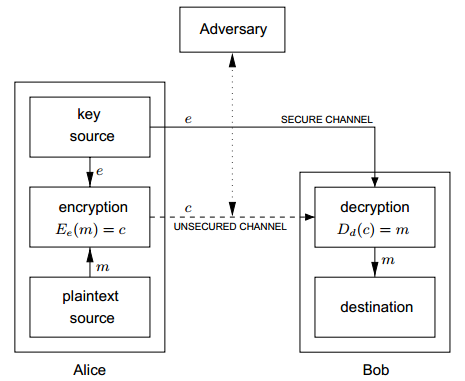
\includegraphics[width=0.7\textwidth]{symmetric-key.png}
	\caption{Two-party communication using symmetric encryption, with a secure channel for key exchange. \citep{menezes_handbook_1996}}
\end{figure}

\section{Block cipher}

"A block cipher is an encryption scheme which breaks up the plaintext messages to be transmitted into strings (called blocks) of a fixed length t over an alphabet $A$, and encrypts one block at a time." \citep{menezes_handbook_1996}

\paragraph{Definition}
"A block cipher is specified by an encryption function which takes as input a key $K$ of bit length $k$, called the key size, and a bit string $P$ of length $n$, called the block size, and returns a string $C$ of $n$ bits. $P$ is called the plaintext, and $C$ is termed the ciphertext. For each $K$, the function $E_K(P)$ is required to be an invertible mapping on $\{0,1\}^{n}$.
$$
E_K(P) := E(K,P): \{0,1\}^k \times \{0,1\}^n \rightarrow \{0,1\}^n
$$
The inverse for $E$ is defined as a function
$$
E_K^{-1}(C) := D_K(C) = D(K,C): \{0,1\}^k \times \{0,1\}^n \rightarrow \{0,1\}^n
$$
taking a key $K$ and a ciphertext $C$ to return a plaintext value $P$, such that
$$
\forall K: D_K(E_K(P)) = P
$$
For each key $K$, $E_K$ is a permutation (a bijective mapping) over the set of input blocks. Each key selects one permutation from the possible set of $(2^n)!$." \citep{wiki:block-cipher}

"A block cipher whose block size $n$ is too small may be vulnerable to attacks based on statistical analysis. One such attack involves simple frequency analysis of ciphertext block. However, choosing too large a value for the blocksize $n$ may create difficulties as the complexity of implementation of many ciphers grows rapidly with block size." \citep{menezes_handbook_1996}

\subsection{Modes of operation}

"A mode of operation is an algorithm that uses a block cipher to encrypt messages of arbitrary length in a way that provides confidentiality or authenticity. A block cipher by itself is only suitable for the secure cryptographic transformation (encryption or decryption) of one fixed-length group of bits called a block. A mode of operation describes how to repeatedly apply a cipher's single-block operation to securely transform amounts of data larger than a block." \citep{wiki:mode-operation}

The four most common modes are ECB, CBC, CFB, and OFB. 

\subsubsection{ECB mode}

"The simplest of the encryption modes is the \textit{Electronic Codebook} (ECB) mode. The message is divided into blocks, and each block is encrypted separately." \citep{wiki:mode-operation}

The algorithm of the mode of operation ECB is the following:

\begin{figure}[!ht]
	\centering
	\label{fig:ecb}
	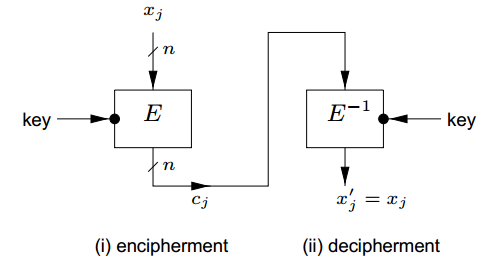
\includegraphics[width=0.7\textwidth]{ecb.png}
	\caption{ECB mode of operation. \citep{menezes_handbook_1996}}
\end{figure}

\paragraph{Algorithm}
ECB mode of operation. \citep{menezes_handbook_1996} \\
INPUT: $k$-bit key $K$; $n$-bit plaintext blocks $x_1, ... , x_t$. \\
SUMMARY: produce ciphertext blocks $c_1, ... , c_t$; decrypt to recover plaintext.
\begin{enumerate}[noitemsep]
\item Encryption: $for\ 1 \le j \le t, c_j \leftarrow E_K(x_j)$.
\item Decryption: $for\ 1 \le j \le t, x_j \leftarrow E_k^{-1}(c_j)$.
\end{enumerate}

"The disadvantage of this method is that identical plaintext blocks are encrypted into identical ciphertext blocks; thus, it does not hide data patterns well." \citep{wiki:mode-operation}

\subsubsection{CBC mode}

"In \textit{Cipher Block Chaining} (CBC) mode, each block of plaintext is XORed with the previous ciphertext block before being encrypted. This way, each ciphertext block depends on all plaintext blocks processed up to that point. To make each message unique, an initialization vector ($IV$) must be used in the first block." \citep{wiki:mode-operation}

The algorithm of the mode of operation CBC is the following:

\begin{figure}[!ht]
	\centering
	\label{fig:cbc}
	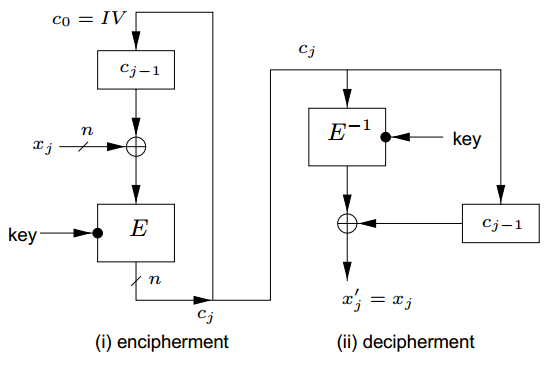
\includegraphics[width=0.7\textwidth]{cbc.png}
	\caption{CBC mode of operation. \citep{menezes_handbook_1996}}
\end{figure}

\paragraph{Algorithm}
CBC mode of operation. \citep{menezes_handbook_1996} \\
INPUT: $k$-bit key $K$; $n$-bit $IV$ ; $n$-bit plaintext blocks $x_1, ... , x_t$. \\
SUMMARY: produce ciphertext blocks $c_1, ... , c_t$; decrypt to recover plaintext.
\begin{enumerate}[noitemsep]
\item Encryption: $c_0 \leftarrow IV.\ For\ 1 \le j \le t, c_j \leftarrow E_K(c_{j-1} \oplus x_j)$.
\item Decryption: $c_0 \leftarrow IV.\ For\ 1 \le j \le t, x_j \leftarrow c_{j-1} \oplus E_{K}^{-1}(c_j)$.
\end{enumerate}

"Its main drawbacks are that encryption is sequential (i.e., it cannot be parallelized), and that the message must be padded to a multiple of the cipher block size." \citep{wiki:mode-operation}

\subsubsection{CFB mode}

"The \textit{Cipher Feedback} (CFB) mode, a close relative of CBC, makes a block cipher into a self-synchronizing stream cipher." \citep{wiki:mode-operation}

"While the CBC mode processes plaintext $n$ bits at a time (using an $n$-bit block cipher), some applications require that $r$-bit plaintext units be encrypted and transmitted without delay, for some fixed $r < n$ (often $r = 1$ or $r = 8$)." \citep{menezes_handbook_1996}

The algorithm of the mode of operation CFB is the following:

\begin{figure}[!ht]
	\centering
	\label{fig:cfb}
	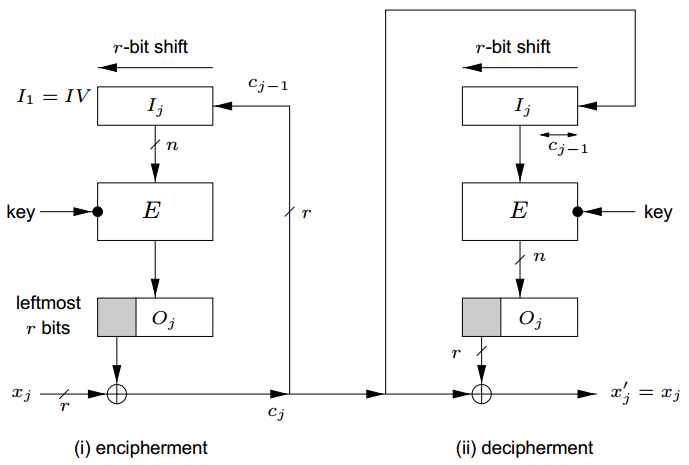
\includegraphics[width=0.7\textwidth]{cfb.png}
	\caption{CFB mode of operation. \citep{menezes_handbook_1996}}
\end{figure}

\paragraph{Algorithm}
CFB-r mode of operation. \citep{menezes_handbook_1996} \\
INPUT: $k$-bit key $K$; $n$-bit $IV$ ; $r$-bit plaintext blocks $x_1, ... , x_u\ (1 \le r \le n)$. \\
SUMMARY: produce ciphertext blocks $c_1, ... , c_u$; decrypt to recover plaintext.
\begin{enumerate}[noitemsep]
\item Encryption: $I_1 \leftarrow IV.$ ($I_j$ is the input value in a shift register). $For\ 1 \le j \le u:$
	\begin{enumerate}
	\item $O_j \leftarrow E_K(I_j).$ (Compute the block cipher output).
	\item $t_j \leftarrow$ the $r$ leftmost bits of $O_j$. (Assume the leftmost is identified as bit 1).
	\item $c_j \leftarrow x_j \oplus t_j.$ (Transmit the r-bit ciphertext block cj).
	\item $I_{j+1} \leftarrow 2^r.\ I_j + c_j\ mod\ 2^n.$ (Shift $c_j$ into right end of shift register).
	\end{enumerate}
\item Decryption: $I_1 \leftarrow IV.\ For\ 1 \le j \le u,$ upon receiving $c_j$:\\
$x_j \leftarrow c_j \oplus t_j,$ where $t_j$, $O_j$ and $I_j$ are computed as above.
\end{enumerate}

"CFB shares two advantages over CBC mode with the stream cipher modes OFB and CTR: the block cipher is only ever used in the encrypting direction, and the message does not need to be padded to a multiple of the cipher block size (though ciphertext stealing can also be used to make padding unnecessary)." \citep{wiki:mode-operation}

\subsubsection{OFB mode}

"The \textit{Output Feedback} (OFB) mode makes a block cipher into a synchronous stream cipher. It generates keystream blocks, which are then XORed with the plaintext blocks to get the ciphertext. Just as with other stream ciphers, flipping a bit in the ciphertext produces a flipped bit in the plaintext at the same location. This property allows many error correcting codes to function normally even when applied before encryption." \citep{wiki:mode-operation}

"Two versions of OFB using an $n$-bit block cipher are common. The ISO version requires an $n$-bit feedback, and is more secure. The earlier FIPS version allows $r < n$ bits of feedback." \citep{menezes_handbook_1996}

The algorithm of the mode of operation OFB is the following:

\paragraph{Algorithm}
OFB mode with full feedback (per ISO 10116). \citep{menezes_handbook_1996} \\
INPUT: $k$-bit key $K$; $n$-bit $IV$ ; $r$-bit plaintext blocks $x_1, ... , x_u\ (1 \le r \le n)$. \\
SUMMARY: produce ciphertext blocks $c_1, ... , c_u$; decrypt to recover plaintext.
\begin{enumerate}[noitemsep]
\item Encryption: $I_1 \leftarrow IV.\ For\ 1 \le j \le u,$ given plaintext block $x_j$:
	\begin{enumerate}
	\item $O_j \leftarrow E_K(I_j).$ (Compute the block cipher output).
	\item $t_j \leftarrow$ the $r$ leftmost bits of $O_j$. (Assume the leftmost is identified as bit 1).
	\item $c_j \leftarrow x_j \oplus t_j.$ (Transmit the r-bit ciphertext block cj).
	\item $I_{j+1} \leftarrow O_j.$ (Update the block cipher input for the next block).
	\end{enumerate}
\item Decryption: $I_1 \leftarrow IV.\ For\ 1 \le j \le u,$ upon receiving $c_j$:\\
$x_j \leftarrow c_j \oplus t_j,$ where $t_j$, $O_j$ and $I_j$ are computed as above.
\end{enumerate}

\paragraph{Algorithm}
OFB mode with r-bit feedback (per FIPS 81). \citep{menezes_handbook_1996} \\
INPUT: $k$-bit key $K$; $n$-bit $IV$ ; $r$-bit plaintext blocks $x_1, ... , x_u\ (1 \le r \le n)$. \\
SUMMARY: produce ciphertext blocks $c_1, ... , c_u$; decrypt to recover plaintext.\\
As per Algorithm ISO 10116, but with $"I_{j+1} \leftarrow O_j"$ replaced by:\\
$I_{j+1} \leftarrow 2^r \cdot I_j + t_j\ mod\ 2^n.$ (Shift output $t_j$ into right end of shift register).

\begin{figure}[!ht]
	\centering
	\label{fig:ofb}
	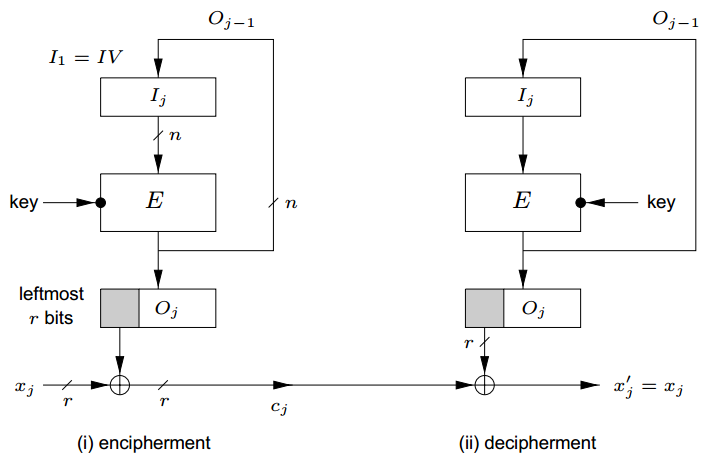
\includegraphics[width=0.7\textwidth]{ofb.png}
	\caption{OFB mode of operation. \citep{menezes_handbook_1996}}
\end{figure}

\section{IDEA cipher}

"The first incarnation of the IDEA cipher, by Xuejia Lai and James Massey, surfaced in 1990. It was called PES (Proposed Encryption Standard). The next year, after Biham and Shamir’s demonstrated differential cryptanalysis, the authors strengthened their cipher against the attack and called the new algorithm IPES (Improved Proposed Encryption Standard). IPES changed its name to IDEA (International Data Encryption Algorithm) in 1992." \citep{schneier_applied_1996}

"IDEA cipher encrypts 64-bit plaintext to 64-bit ciphertext blocks, using a 128-bit input key $K$. Based in part on a novel generalization of the Feistel structure, it consists of 8 computationally identical rounds followed by an output transformation. Round $r$ uses six 16-bit subkeys $K_{i}^{(r)},\ 1 \le i\le 6$, to transform a 64-bit input $X$ into an output of four 16-bit blocks, which are input to the next round. The round 8 output enters the output transformation, employing four additional subkeys $K_{i}^{(9)},\ 1 \le i \le 4$ to produce the final ciphertext $Y = (Y_1, Y_2, Y_3, Y_4)$. "The same algorithm is used for both encryption and decryption." \citep{schneier_applied_1996}

All subkeys are derived from $K$. A dominant design concept in IDEA is mixing operations from three different algebraic groups of $2^n$ elements. The corresponding group operations on sub-blocks $a$ and $b$ of bitlength $n = 16$ are:" \citep{menezes_handbook_1996} 
\begin{itemize}[noitemsep]
	\item $a \oplus b$: bitwise XOR. 
	\item $a \boxplus b$: addition $mod\ 2^n$: $(a+b)\ AND\ 0xFFFF$.
	\item $a \odot b$: (modified) multiplication $mod\ 2^n+1$, with $0 \in Z_{2^n}$ associated with $2^n \in Z_{2^{n+1}}$.
\end{itemize}

\begin{figure}[!ht]
	\centering
	\label{fig:idea}
	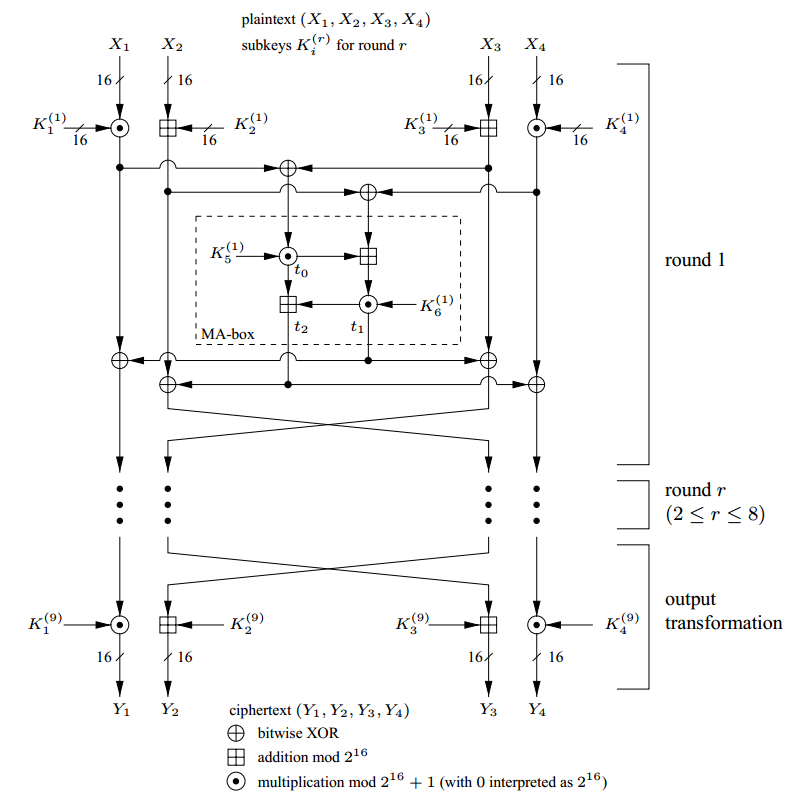
\includegraphics[width=0.92\textwidth]{idea.png}
	\caption{IDEA computation path. \citep{menezes_handbook_1996}}
\end{figure}

"The 64-bit data block is divided into four 16-bit sub-blocks: $X_1$, $X_2$, $X_3$ and $X_4$. These four sub-blocks become the input to the first round of the algorithm. There are eight rounds total. In each round the four sub-blocks are XORed, added, and multiplied with one another and with six 16-bit subkeys. Between rounds, the second and third sub-blocks are swapped. 

Finally, the four sub-blocks are combined with four subkeys in an output transformation.

In each round, the sequence of events is as follows:

\begin{enumerate}[noitemsep]
	\item Multiply $X_1$ and the first subkey.
	\item Add $X_2$ and the second subkey.
	\item Add $X_3$ and the third subkey.
	\item Multiply $X_4$ and the fourth subkey.
	\item XOR the results of steps (1) and (3).
	\item XOR the results of steps (2) and (4). 
	\item Multiply the results of step (5) with the fifth subkey. 
	\item Add the results of steps (6) and (7). 
	\item Multiply the results of step (8) with the sixth subkey. 
	\item Add the results of steps (7) and (9). 
	\item XOR the results of steps (1) and (9). 
	\item XOR the results of steps (3) and (9). 
	\item XOR the results of steps (2) and (10). 
	\item	XOR the results of steps (4) and (10). 
\end{enumerate}

"The output of the round is the four sub-blocks that are the results of steps  (11), (12), (13), and (14). Swap the two inner blocks (except for the last round) and that is the input to the next round. 

After the eighth round, there is a final output transformation:

\begin{enumerate}[noitemsep]
	\item Multiply $X_1$ and the first subkey.
	\item Add $X_2$ and the second subkey.
	\item Add $X_3$ and the third subkey.
	\item Multiply $X_4$ and the fourth subkey.
\end{enumerate}

Finally, the four sub-blocks are reattached to produce the ciphertext.

Creating the subkeys is also easy. The algorithm uses 52 of them (six for each of the eight rounds and four more for the output transformation). First, the 128-bit key is divided into eight 16-bit subkeys. These are the first eight subkeys for the algorithm (the six for the first round, and the first two for the second round). Then, the key is rotated 25 bits to the left and again divided into eight subkeys. The first four are used in round 2; the last four are used in round 3. The key is rotated another 25 bits to the left for the next eight subkeys, and so on until the end of the algorithm." \citep{schneier_applied_1996}

"The very simple key schedule makes IDEA subject to a class of weak keys; some keys containing a large number of 0 bits produce weak encryption.[9] These are of little concern in practice, being sufficiently rare that they are unnecessary to avoid explicitly when generating keys randomly." \citep{wiki:idea}

"Decryption is exactly the same, except that the subkeys are reversed and slightly different. The decryption subkeys are either the additive or multiplicative inverses of the encryption subkeys. (For the purposes of IDEA, the all-zero sub-block is considered to represent $2^16 = –1$ for multiplication 
modulo $2^{16} + 1$; thus the multiplicative inverse of 0 is 0). Calculating these takes some doing, but you only have to do it once for each decryption key." \citep{schneier_applied_1996}

\begin{figure}[!ht]
	\centering
	\label{fig:idea-enc}
	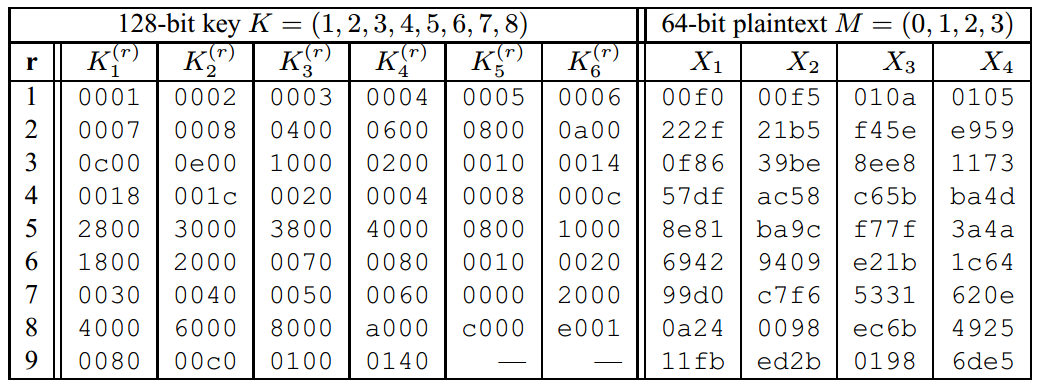
\includegraphics[width=\textwidth]{idea-enc.png}
	\caption{IDEA encryption sample. \citep{menezes_handbook_1996}}
\end{figure}

\begin{figure}[!ht]
	\centering
	\label{fig:idea-dec}
	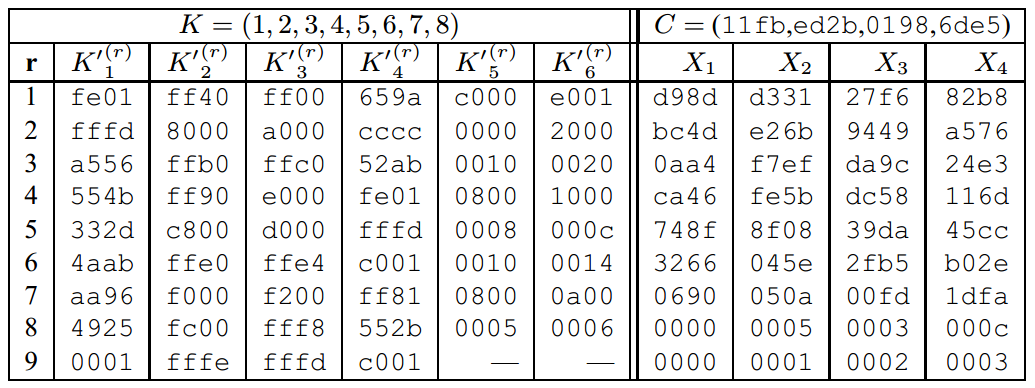
\includegraphics[width=\textwidth]{idea-dec.png}
	\caption{IDEA decryption sample. \citep{menezes_handbook_1996}}
\end{figure}

% -------------------------------------------------------------
% Bibliography
% -------------------------------------------------------------
\newpage
\bibliography{citations}
\bibliographystyle{plainnat}

\end{document}